\documentclass[12pt]{article}
\usepackage[margin=3cm]{geometry}
\usepackage{graphicx}
\usepackage{float}

\begin{document}

\begin{titlepage}
	\begin{center}
		
		
		% Upper part of the page. The '~' is needed because \\
		% only works if a paragraph has started.
		\vfill
		
		\textsc{\LARGE Lab 2: Inverter Schematic}\\[1.5cm]
		
		\Large Adam Sumner\\[0.5cm]
		
		\Large Illinois Insititute of Technology\\[0.5cm]
		
		\Large ECE 429-01\\[0.5cm]	
		
		\noindent
		\vfill
		\large \textbf{Lab Date:} September 21\textsuperscript{st}, 2015\hfill
		\large \textbf{Due Date:} September 28\textsuperscript{th}, 2015
		% Bottom of the page
		
		
	\end{center}
\end{titlepage}

\section{Introduction}
The purpose of this lab is to introduce the student to the various tools that will be used throughout the semester. The student will design a schematic of a CMOS inverter, create the inverter in Virtuoso, and test the correctness of the design using HSPICE.

\section{Theory/Pre-Lab}
\subsection{Theory}
Due to the costly nature of manufacturing VLSI chips and the difficulty of testing devices on the nanoscale level, a majority of VLSI design work is done using computers and simulation  software. Designers rely heavily on CAD techniques to validate their designs before the designs are pushed into production. The Cadence Virtuoso platform is one of the most widely used commercial electronic design automation platform that supports custom IC designs. It serves as a central point for design entry, and it also provides various interfaces for use with other EDA tools. Throughout this lab, the FreePDK45 library, which supports a 45 nm process derived from the Predictive Technology Model, will be used.

Complementary MOSFET or CMOS technology is widely used in industry today. Devices ranging from Cell phones to CPU's all utilize CMOS due to its advantages over pure NMOS or pure PMOS designs. CMOS offers devices low power dissipation, relatively high speed, and high noise margins in both states. The most basic logic gate that can be implemented using CMOS is an inverter. This involves the use of only 2 MOSFETs, one PMOS type and one NMOS type. Figure \ref{fig:inverter} shows the layout of a CMOS inverter. 
\begin{figure}[H]
\centering
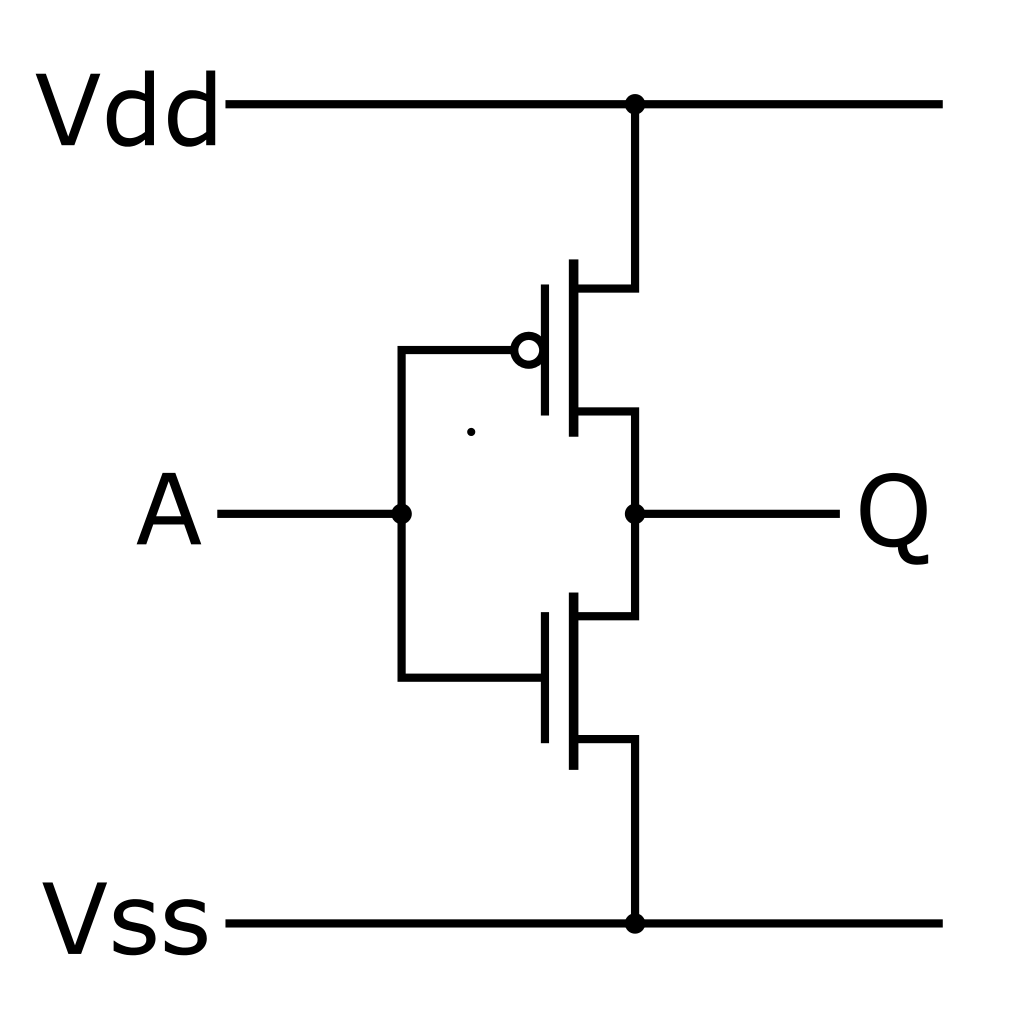
\includegraphics[width=0.4\linewidth]{inverter}
\caption{CMOS Inverter Schematic}
\label{fig:inverter}
\end{figure}


\subsection{Pre-Lab}
The pre-lab involved a refreshment of the various SPICE netlists, an overview of Tutorial I: Inverter Schematic and Simulation, and the creation of a schematic for a static CMOS inverter with power sources connected. The drawn schematic is shown below in Figure \ref{fig:prelab}:
\begin{figure}[H]
\centering
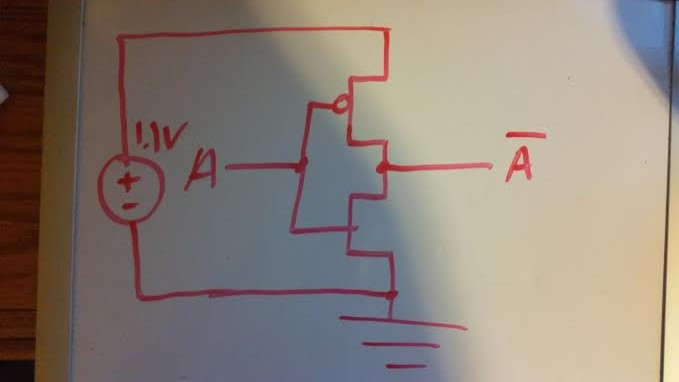
\includegraphics[width=0.5\linewidth]{prelab}
\caption{Static CMOS Inverter with Power Source}
\label{fig:prelab}
\end{figure}

\section{Implementation}
\subsection{Schematics}
\begin{figure}[H]
\centering
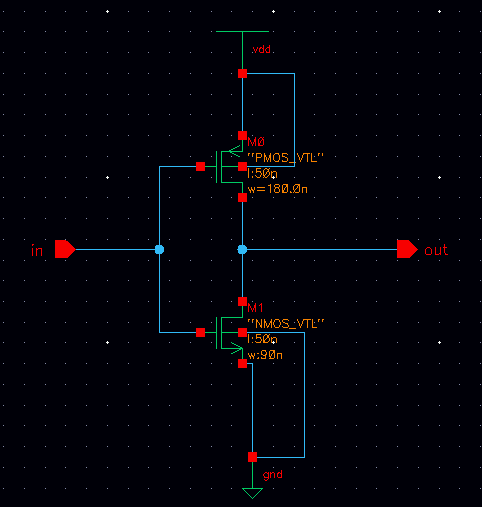
\includegraphics[width=0.5\linewidth]{custom_inverter}
\caption{Custom CMOS Inverter Schematic}
\label{fig:custom_inverter}
\end{figure}

\begin{figure}[H]
\centering
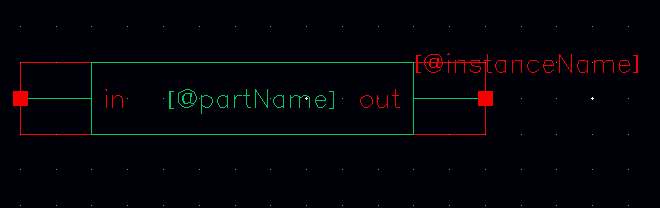
\includegraphics[width=0.7\linewidth]{custom_symbol}
\caption{Custom CMOS Inverter Symbol}
\label{fig:custom_symbol}
\end{figure}

\begin{figure}[H]
\centering
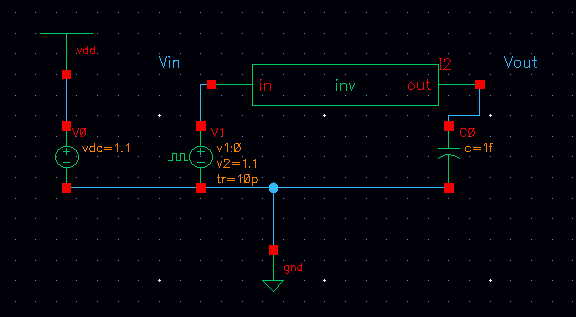
\includegraphics[width=0.7\linewidth]{lab2_schematic}
\caption{Schematic Created for Simulation}
\label{fig:lab2_schematic}
\end{figure}

\subsection{Procedure}
This lab first involved creating an inverter with the PMOS component width of 180 nm and the NMOS component with a width of 80 nm. This schematic is shown in Figure \ref{fig:custom_inverter}. Once created, a symbol was then generated for the schematic so that a test circuit could be created to test the functionality of the created inverter. The symbol is shown in Figure \ref{fig:custom_symbol}, and the test circuit is shown in Figure \ref{fig:lab2_schematic}. For the input to the inverter, a square wave was used with a max voltage level of 1.1V and a min voltage level of 0V. A simulation was then performed and $V_{in}$ vs $V_{out}$ of the input to the inverter was analyzed. The results are shown in Figure \ref{fig:graph}. The delay of the inverter was then calculated using the measurement tool. These results are shown in Figure \ref{fig:delay}.

\subsection{Results}
\begin{figure}[H]
\centering
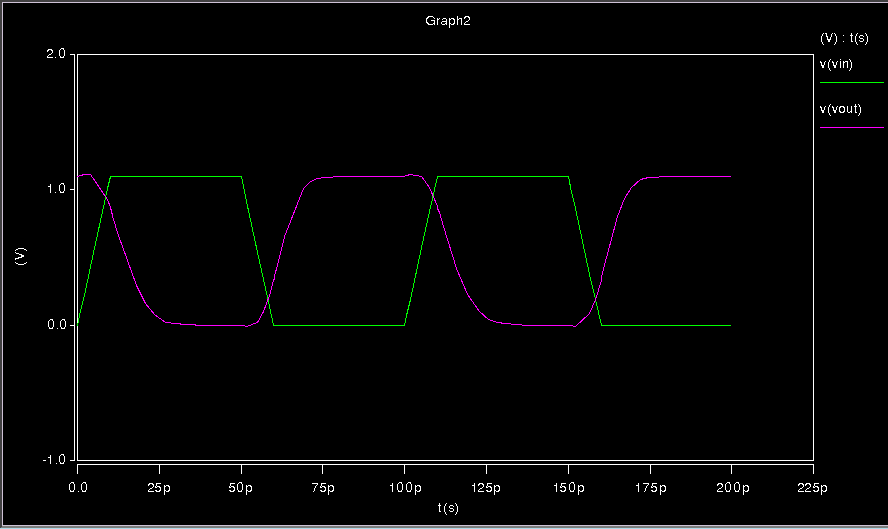
\includegraphics[width=0.7\linewidth]{graph}
\caption{Inverter Simulation Results: $V_{in}$ vs $V_{out}$}
\label{fig:graph}
\end{figure}

\begin{figure}[H]
\centering
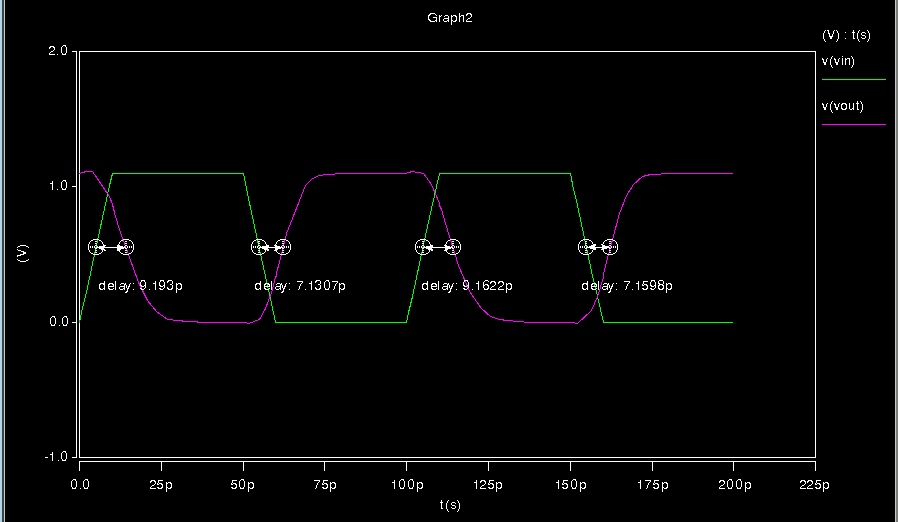
\includegraphics[width=0.7\linewidth]{delay}
\caption{Inverter Delay}
\label{fig:delay}
\end{figure}

\subsection{Discussion}
This lab primarily served as an introduction to the tools that will be used throughout the semester. Because of this, the results obtained in this lab were easily produced with the guide of the Lab 2 Tutorial document. The expected waveforms were produced, along with the expected time delay associated with the specifications of this inverter schematic. It is clear in Figure \ref{fig:graph} that $V_{in}$ has the proper waveform specified in the schematic. It is also clear that  $V_{out}$ is not an exact inverse representation of $V_{in}$, but this is due to propogation delay, an unavoidable side effect of digital circuit design.
\subsection{Questions}
\begin{enumerate}
	\item \textbf{Where are the bodies of the transistors in your schematic?} \\
	The body of the PMOS transistor is located in the middle right and is connected to $V_{dd}$. The body of the NMOS transistor is located in the middle right and is connected to GND. These can easily be seen in Figure \ref{fig:custom_inverter}
	
	\item \textbf{What are the widths and lengths of your transistors?}\\
	For PMOS, the width is 180nm and the length is 50nm. For NMOS, the width is 90nm and the length is 50nm.
	
	\item \textbf{How much is the supply voltage?}\\
	1.1V
	
	\item \textbf{What do ‘Rise time’ and ‘Pulse width’ mean for ‘vpulse’ ? Can you locate these two values in the waveforms obtained from the SPICE simulation?} \\
	The rise time refers to the time it takes for the voltage to rise from $V_{min}$ to $V_{max}$. For \texttt{vpulse} this value is 10 ps. The pulse width refers to how long $V_{max}$ is applied. For \texttt{vpulse} this value is 40 ps. In our case, the rise time is also equal to the fall time of our wave, giving the input wave a total period of 100 ps.
	
	\item \textbf{Tutorial I shows a maximum rising delay of 7.1892p. How long is that in seconds?}\\
	7.1892p is equivalent to $7.1892 \times 10^{-12}$ seconds
	
	\item \textbf{To obtain an inverter design with equal rising and falling delays, will you make the PMOS transistor larger or smaller?}\\
	The PMOS transistor should be larger than the NMOS transistor by roughly 2 or 3 times because this will result in the rise and fall time being equivalent 
\end{enumerate}
%\subsection{Bonus Work}
\section{Conclusions}
Overall this lab was a success. A CMOS inverter schematic was successfully created, a test circuit was designed and simulated, and the results were recorded and in agreement with the expected values. This schematic can be used to obtain accurate results in further labs conducted and in other circuit designs.
\end{document}
